\documentclass[a4paper, 12pt]{article}

\usepackage{hyperref}
\usepackage[warn]{mathtext}
\usepackage[utf8]{inputenc}
\usepackage[T2A]{fontenc}
\usepackage[english,russian]{babel}
\usepackage{multirow}
\usepackage{amsmath,amsfonts,amssymb,amsthm,mathtools}
\usepackage{indentfirst}
\DeclareSymbolFont{T2Aletters}{T2A}{cmr}{m}{it}
\usepackage{ gensymb }
\mathtoolsset{showonlyrefs=true}
\usepackage{euscript}
\usepackage{mathrsfs}
\usepackage[left=2cm,right=2cm,top=2cm,bottom=2cm]{geometry}
\usepackage{graphicx}
\usepackage{wrapfig}
\usepackage[rgb]{xcolor}
\hypersetup{
colorlinks=true,
urlcolor=blue
}


\title{Лабораторная работа}
\author{Гисич Арсений Б03-109}
\date{2022}

\begin{document}

	\begin{center}
		{\large МОСКОВСКИЙ ФИЗИКО-ТЕХНИЧЕСКИЙ ИНСТИТУТ (НАЦИОНАЛЬНЫЙ ИССЛЕДОВАТЕЛЬСКИЙ УНИВЕРСИТЕТ)}
	\end{center}
	\vspace{5 cm}
	{\Large
		\begin{center}
			{\bf Лабораторная работа 2.2.3}\\[0.2 cm]
			Измерение теплопроводности воздуха при атмосферном давлении
		\end{center}
	}
	\vspace{4 cm}
	\begin{flushright}
		{\Large Выполнил: \\
			\vspace{0.2 cm}
			Гисич Арсений \\
			\vspace{0.2 cm}
			Б03-109 \\}
	\end{flushright}
	\vspace{8 cm}
	\begin{center}
		Долгопрудный\\[0.1 cm]
		2022
	\end{center}
\thispagestyle{empty}

\section{Аннотация}

\par Цель работы: измерить коэффициент теплопроводности воздуха при атмосферном
давлении в зависимости от температуры.

\section{Теоретические сведения}

\textit{Теплопроводность} — это процесс передачи тепловой энергии от нагретых частей системы к холодным за счёт хаотическогодвижения частиц среды(молекул, атомов и т.п.). В газах теплопроводность осуществляется за счёт непосредственной передачи кинетической энергии от быстрых молекул к медленным при их столкновениях. Перенос тепла описывается законом Фурье, утверждающим, что плотность потока энергии $\vec{q} \: [\frac{Вт}{м^{2}}]$ (количество теплоты, перено-симое   через единичную площадку в единицу времени) пропорциональна градиенту температуры:
\begin{equation}\label{1}
	\vec{q} = -\kappa \cdot \nabla T,
\end{equation}
где $\kappa$ — \textit{коэффициент теплопроводности}.

\begin{equation}\label{2}
	\kappa \sim \lambda \vec{\nu} \cdot n c_v,
\end{equation}
где $\lambda$  — длина свободного пробега молекул газа, $\vec{v}$ — средняя скорость их теплового движения, n — концентрация (объёмная плотность) газа.

Решая дифференциальное уравнение для цилиндического случая получаем:
\begin{equation}\label{3}
	Q = \frac{2\pi L}{ln\frac{r_0}{r_1}} \kappa \cdot \Delta T.
\end{equation}

\section{Методика измерений}

\begin{wrapfigure}{r}{0.3\textwidth}
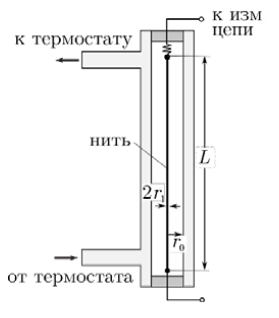
\includegraphics[width=0.3\textwidth]{1.png}
\caption{Схема установки}
\label{ris1}
\end{wrapfigure}

На оси полой цилиндрической трубки с внутреннимдиаметром $2r_0=(1,00\pm0,01)см$ размещена металлическая нить диаметром $2r_1=(0,055\pm0,005)мм$ и длиной $L=(365\pm2)мм$ (материал нити и точные геометрические размеры указаныв техническом описании установки). Полость трубки заполнена воздухом (полость через небольшое отверстие сообщается с атмосферой). Стенки трубки помещены в кожух, через которых пропускается вода из термостата, так что их температура поддерживается постоянной. Для предотвращения конвекции трубка  расположена вертикально.

Металлическая нить служит как источником тепла, так и датчиком температуры (термометром сопротивления). По пропускаемому через нить постоянному току I и напряжению U на ней вычисляется мощность нагрева по закону Джоуля–Ленца:
\begin{equation}\label{4}
	Q = UI,
\end{equation}
и сопротивление по закону Ома:
\begin{equation}\label{5}
	R = \frac{U}{I}.
\end{equation}

Сопротивление нити является однозначной функцией её температуры $R(t)$. Для большинства металлов относительное изменение сопротивления из-за нагрева невелико: приизменении температуры на 1 градус относительное изменение сопротивления нити может составлять приблизительно от 0,2 \% до 0,6\% (в зависимости от её материала).Следовательно, измерение R важно провести с высокой точностью.

\begin{wrapfigure}{r}{0.55\textwidth}
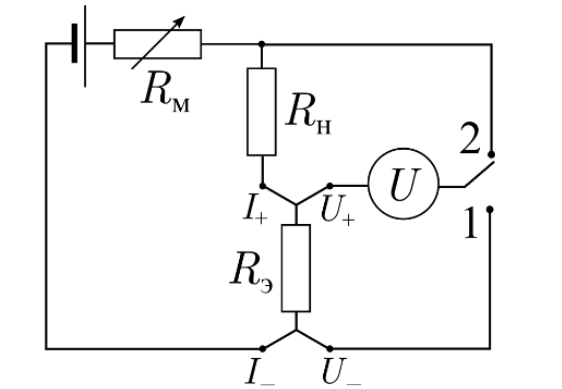
\includegraphics[width=0.5\textwidth]{2.png}
\caption{Электрическая схема измерения сопротивления нити и мощности нагрева}
\label{ris2}
\end{wrapfigure}

Схема предусматривает использование одного вольтметра и эталонного сопротивления $R_э\sim10 \: Ом$, включённого последовательно с нитью. В положении переключателя 2 вольтметр измеряет напряжение на нити, а в положении 1 — напряжениена $R_э$, пропорциональное токучерез нить. Для исключения влияния контактов и подводящих проводов эталонное сопротивление $R_э$ также   необходимо подключать в цепь по четырёхпроводной схеме.
Ток в цепи в обеих схемах регулируется с помощью реостата или магазина сопротивлений $R_м$, включённого последовательно с источником напряжения.

В исследуемоминтервалетемператур $(20–70~\celsius)$ зависимость сопротивления  от температуры можно с хорошей точностью аппроксимировать линейной функцией:
\begin{equation}\label{6}
	R(t) = R_{273} \cdot (1+\alpha t),
\end{equation}
где t — температурав [$\celsius$], $R_{273}$ — сопротивление нити при температуре $20~\celsius$ и \\ $\alpha = \frac{1}{R_{273}}\frac{dR}{dT}$ — температурный коэффициент сопротивления материала.


\section{Используемое оборудование}

\begin{enumerate}
    \item цилиндрическая колба с натянутой по оси нитью;
    \item термостат;
    \item источник питания постоянного тока;
    \item амперметр, вольтметр (цифровые мультиметры), $\delta_{А} = 0,005~А$;
    \item эталонное сопротивление;
    \item источник постоянного напряжения;
    \item магазин сопротивлений;
\end{enumerate}

\section{Результаты измерений и обработка данных}

Начальные условия:

$\begin{aligned}
& T = 23,1\pm0,1~\celsius
\end{aligned}$\\[0,5 cm]

Проведём предварительные расчёты парметров опыта. Принимая $\Delta{t_{max}} = 10~\celsius$, \\ $\kappa \sim 25~мВт/(м\cdot{K})$, получаем $$Q = 110~мВт; \quad I = \sqrt{\frac{Q}{R}} = 105~мА.$$

Результаты измерений $R(Q)$ представленны в таб. \ref{tab1}-\ref{tab4}.

\begin{table}[h!]
\begin{center}
\begin{tabular}{|c|c|c|c|c|c|c|c|}
\hline
$I, A$ & $\delta_I, A$ & $U, B$  & $\delta_U, B$ & $Q, Вт$ & $\delta_Q, Вт$ & $R, Ом$ & $\delta_R, Ом$ \\ \hline
0,05   & 0,005         & 0,57190 & 0,00003       & 0,0286  & 0,0029         & 11,44   & 1,14           \\ \hline
0,04   & 0,005         & 0,46558 & 0,00002       & 0,0186  & 0,0023         & 11,64   & 1,45           \\ \hline
0,03   & 0,005         & 0,36405 & 0,00002       & 0,0109  & 0,0018         & 12,14   & 2,02           \\ \hline
0,02   & 0,005         & 0,26005 & 0,00001       & 0,0052  & 0,0013         & 13,00   & 3,25           \\ \hline
0,01   & 0,005         & 0,14615 & 0,00001       & 0,0015  & 0,0007         & 14,62   & 7,31           \\ \hline
0,11   & 0,005         & 1,17080 & 0,00009       & 0,1288  & 0,0059         & 10,64   & 0,48           \\ \hline
0,08   & 0,005         & 0,80057 & 0,00003       & 0,0640  & 0,0040         & 10,01   & 0,63           \\ \hline
\end{tabular}
\caption{$T_1 = 23,1~\celsius$}
\label{tab1}
\end{center}
\end{table}

\begin{table}[h!]
\begin{center}
\begin{tabular}{|c|c|c|c|c|c|c|c|}
\hline
$I, A$ & $\delta_I, A$ & $U, B$  & $\delta_U, B$ & $Q, Вт$ & $\delta_Q, Вт$ & $R, Ом$ & $\delta_R, Ом$ \\ \hline
0,01   & 0,005         & 0,16042 & 0,00001       & 0,0016  & 0,0008         & 16,04   & 8,02           \\ \hline
0,02   & 0,005         & 0,23591 & 0,00001       & 0,0047  & 0,0012         & 11,80   & 2,95           \\ \hline
0,03   & 0,005         & 0,30849 & 0,00002       & 0,0093  & 0,0015         & 10,28   & 1,71           \\ \hline
0,04   & 0,005         & 0,44552 & 0,00002       & 0,0178  & 0,0022         & 11,14   & 1,39           \\ \hline
0,07   & 0,005         & 0,74165 & 0,00003       & 0,0519  & 0,0037         & 10,60   & 0,76           \\ \hline
0,08   & 0,005         & 0,80061 & 0,00003       & 0,0640  & 0,0040         & 10,01   & 0,63           \\ \hline
0,10   & 0,005         & 1,05017 & 0,00009       & 0,1050  & 0,0053         & 10,50   & 0,53           \\ \hline
\end{tabular}
\caption{$T_2 = 35~\celsius$}
\label{tab2}
\end{center}
\end{table}

\begin{table}[h!]
\begin{center}
\begin{tabular}{|c|c|c|c|c|c|c|c|}
\hline
$I, A$ & $\delta_I, A$ & $U, B$  & $\delta_U, B$ & $Q, Вт$ & $\delta_Q, Вт$ & $R, Ом$ & $\delta_R, Ом$ \\ \hline
0,01   & 0,005         & 0,16850 & 0,00001       & 0,0017  & 0,0008         & 16,85   & 8,43           \\ \hline
0,02   & 0,005         & 0,25384 & 0,00001       & 0,0051  & 0,0013         & 12,69   & 3,17           \\ \hline
0,03   & 0,005         & 0,33987 & 0,00002       & 0,0102  & 0,0017         & 11,33   & 1,89           \\ \hline
0,05   & 0,005         & 0,51401 & 0,00002       & 0,0257  & 0,0026         & 10,28   & 1,03           \\ \hline
0,08   & 0,005         & 0,80056 & 0,00003       & 0,0640  & 0,0040         & 10,01   & 0,63           \\ \hline
0,09   & 0,005         & 0,95146 & 0,00004       & 0,0856  & 0,0048         & 10,57   & 0,59           \\ \hline
0,11   & 0,005         & 1,17099 & 0,00005       & 0,1288  & 0,0059         & 10,65   & 0,48           \\ \hline
\end{tabular}
\caption{$T_3 = 45~\celsius$}
\label{tab3}
\end{center}
\end{table}

\newpage

\begin{table}[h!]
\begin{center}
\begin{tabular}{|c|c|c|c|c|c|c|c|}
\hline
$I, A$ & $\delta_I, A$ & $U, B$  & $\delta_U, B$ & $Q, Вт$ & $\delta_Q, Вт$ & $R, Ом$ & $\delta_R, Ом$ \\ \hline
0,01   & 0,005         & 0,14146 & 0,00001       & 0,0014  & 0,0007         & 14,15   & 7,07           \\ \hline
0,02   & 0,005         & 0,21795 & 0,00001       & 0,0044  & 0,0011         & 10,90   & 2,72           \\ \hline
0,04   & 0,005         & 0,47411 & 0,00002       & 0,0190  & 0,0024         & 11,85   & 1,48           \\ \hline
0,05   & 0,005         & 0,53708 & 0,00002       & 0,0269  & 0,0027         & 10,74   & 1,07           \\ \hline
0,07   & 0,005         & 0,73055 & 0,00003       & 0,0511  & 0,0037         & 10,44   & 0,75           \\ \hline
0,09   & 0,005         & 0,88960 & 0,00004       & 0,0801  & 0,0044         & 9,88    & 0,55           \\ \hline
0,11   & 0,005         & 1,13321 & 0,00009       & 0,1247  & 0,0057         & 10,30   & 0,47           \\ \hline
\end{tabular}
\caption{$T_4 = 70~\celsius$}
\label{tab4}
\end{center}
\end{table}



\section{Обсуждение результатов и выводы}

В данной работе исследовалась зависимость повышения температуры воздуха от мощности подводимого тепла и расхода при стационарном течении через трубку. По результатам измерений определялась удельная теплоёмкость воздуха при постоянном давлении. Полученное значение:
$$\boxed{c_p = 837,01\pm160,91~\frac{Дж}{кг \cdot K}}.$$
Использованный в работе метод измерений позволяет достичь относительной точности результатов в 19\%. Полученный результат согласуется с табличным значением --- $1003~\frac{Дж}{кг \cdot K}$. Основной вклад в погрешность вносит погрешность определения расхода.
Также в данной работе была определена доля тепловых потерь:
$$\boxed{\frac{N_{пот}}{N} = 0,29\pm0,06}.$$

\end{document}